\documentclass[12pt,a4paper]{article}
\usepackage{geometry}
\usepackage{graphicx}
\usepackage{float}
\usepackage{hyperref}
\usepackage{amsmath}
\usepackage{booktabs}
\usepackage{enumitem}
\usepackage{xcolor}
\usepackage{listings}
\usepackage{fancyhdr}
\usepackage{url}
\usepackage{titlesec}
\usepackage{microtype}
\usepackage{parskip}
\usepackage{appendix}
\usepackage{lmodern}
\geometry{margin=1in}

\setlength{\headheight}{15pt}
\addtolength{\topmargin}{-2.5pt}
\pagestyle{fancy}
\fancyhf{}
\lhead{Real-Time Embedded Systems}
\rhead{Transaction Processing System}
\rfoot{Page \thepage}

\setlength{\parindent}{0pt}    % No paragraph indentation
\setlength{\parskip}{8pt}      % Space between paragraphs


% Colors for code listings
\definecolor{codegreen}{rgb}{0,0.6,0}
\definecolor{codegray}{rgb}{0.5,0.5,0.5}
\definecolor{codepurple}{rgb}{0.58,0,0.82}
\definecolor{backcolour}{rgb}{0.95,0.95,0.92}

% Code listing style
\lstdefinestyle{mystyle}{
    backgroundcolor=\color{backcolour},   
    commentstyle=\color{codegreen},
    keywordstyle=\color{magenta},
    numberstyle=\tiny\color{codegray},
    stringstyle=\color{codepurple},
    basicstyle=\ttfamily\footnotesize,
    breakatwhitespace=false,         
    breaklines=true,                 
    captionpos=b,                    
    keepspaces=true,                 
    numbers=left,                    
    numbersep=5pt,                  
    showspaces=false,                
    showstringspaces=false,
    showtabs=false,                  
    tabsize=2
}
\lstset{style=mystyle}

% Colors for document
\definecolor{sectcolor}{RGB}{70,30,80}
\definecolor{linkcolor}{RGB}{0,120,215} 
\definecolor{tableheader}{RGB}{240,240,255}

% Section formatting
\titleformat{\section}
  {\normalfont\Large\bfseries\color{sectcolor}}{\thesection}{1em}{}
\titleformat{\subsection}
  {\normalfont\large\bfseries\color{sectcolor}}{\thesubsection}{1em}{}

% Hyperref setup
\hypersetup{
    colorlinks=true,
    linkcolor=linkcolor,
    urlcolor=linkcolor,
    pdfborder={0 0 0},
}

% List formatting
\setlist{itemsep=4pt, topsep=6pt}

% Document information
\title{\huge \textbf{Real-Time Transaction Processing System for Raspberry Pi}}
\author{Fraidakis Ioannis\\
\small Department of Electrical and Computer Engineering\\
\small Aristotle University of Thessaloniki}
\date{September 2025}

\begin{document}

\maketitle

\begin{abstract}
This report details the design, implementation, and performance evaluation of a real-time transaction processing system for cryptocurrency trading on a Raspberry Pi platform. The system subscribes to OKX WebSocket streams for eight major cryptocurrency pairs, performing live computations of volume-weighted average prices (VWAP) and cross-asset correlations, while ensuring continuous, stable operation. Employing a multi-threaded producer-consumer architecture with clock\_nanosleep-based scheduling and dynamic deadline compensation, the system achieves precise minute-boundary task execution and robust timing guarantees.
\end{abstract}

\vspace{3mm}

\section{Introduction and Objectives}

\subsection{Project Overview}

The expansion of cryptocurrency markets has generated substantial demand for real-time processing systems capable of analyzing high-frequency trading data streams with minimal latency. This project implements a comprehensive \emph{real-time} transaction processing system targeting the Raspberry Pi platform, demonstrating that sophisticated financial data processing can be achieved on resource-constrained embedded systems. Real-time systems are characterized by their requirement to produce outputs within strict temporal constraints, where delayed responses may invalidate computational results or trading decisions. This implementation addresses the challenge of maintaining temporal guarantees while processing continuous data streams from cryptocurrency exchanges, computing statistical metrics, and performing correlation analysis across multiple trading pairs.


\subsection{System Requirements}

The system specification defines three primary computational tasks:

\begin{itemize}
    \item \textbf{Task 1 (Continuous):} Each incoming trade event must be logged immediately to persistent storage, maintaining a complete audit trail of market activity.

    \item \textbf{Task 2 (Per-Minute):} For each symbol, calculate the volume-weighted average price (VWAP) and total traded volume over the preceding 15-minute window.
    
    \item \textbf{Task 3 (Per-Minute):} For each symbol, compute the Pearson correlation of its last eight 1-minute VWAP values against the historical VWAP sequences of all other symbols, identifying the time of maximum correlation within a 60-minute lag.    
\end{itemize}


\subsection{Target Platform and Constraints}

The implementation targets the following hardware and software environment:

\begin{itemize}

\item \textbf{Hardware:} Raspberry Pi Zero W (ARMv6, 512MB RAM, single core)

\item \textbf{Language:} C (no garbage collection)

\item \textbf{External Dependencies:} libwebsockets library for network communication

\item \textbf{Data Source:} OKX WebSocket API (\texttt{wss://ws.okx.com:8443/ws/v5/public})

\item \textbf{Monitored Instruments:} Eight cryptocurrency pairs (BTC-USDT, ETH-USDT, ADA-USDT, DOGE-USDT, XRP-USDT, SOL-USDT, LTC-USDT, BNB-USDT)

\end{itemize}

Performance requirements include minimizing both processing delay ($t_{\text{written}} - t_{\text{received}}$) and scheduling drift ($t_{\text{executed}} - t_{\text{scheduled}}$)


\section{System Design and Architecture}

\subsection{Thread Architecture and Concurrency Model}

The system implements a multi-threaded architecture optimized for concurrent data processing and real-time responsiveness. This design separates network I/O, data processing, and computational tasks into independent execution contexts, preventing blocking operations from affecting system timing. The architecture comprises five specialized threads, each responsible for distinct system functions:

\begin{enumerate}
    \item \textbf{WebSocket Thread (Producer):} Manages the connection to the OKX WebSocket server using \texttt{libwebsockets}. Its sole responsibility is to receive incoming trade messages, record the receive timestamp, and push them as raw text into a shared, thread-safe ring buffer (minimal processing, see Section~\ref{sec:Minimal WebSocket Processing}). It also handles connection errors and automatic reconnection with an exponential backoff strategy.
    \item \textbf{Trade Processor Thread (Consumer):} Fetches raw trade messages from the queue, parses the JSON payload to extract trade details, logs the raw transaction (Task 1), and updates the in-memory 15-minute sliding window for current symbol.
    \item \textbf{Scheduler Thread (Coordinator):} Uses \texttt{clock\_nanosleep} with absolute scheduling  to wake up precisely on the minute. Incorporates dynamic deadline compensation using an exponential moving average of computation duration to adjust wake-up times and minimize drift. It coordinates the two worker threads using barriers.
    \item \textbf{VWAP Worker Thread (Worker):} This thread remains blocked until released by the Scheduler's barrier. Once signaled, it computes the 15-min VWAP and volume for all symbols (Task 2), writes results to file, and updates history buffer.   
    \item \textbf{Correlation Worker Thread (Worker):} Also synchronizes with the scheduler via a barrier and runs concurrently with the VWAP worker. It performs Pearson correlation analysis (Task 3) using the latest available data and saves the results. If it accesses a symbol's history before the VWAP worker has updated it, it will use the previous minute's VWAP data, resulting in slightly outdated correlation results. This minor reduction in accuracy enables parallelism and I/O overlap, significantly improving performance compared to strictly sequential execution (see Section~\ref{sec:Concurrency on Single Core}).
    
\end{enumerate}

\subsection{Synchronization}

POSIX thread primitives ensure data consistency and coordinate execution:

\begin{itemize}
    \item \textbf{Mutexes (\texttt{pthread\_mutex\_t}):} Protect shared data structures like the raw trade queue, sliding windows, and VWAP history from race conditions.
    \item \textbf{Condition Variables (\texttt{pthread\_cond\_t}):} Used with the ring queue to allow the trade processor thread to sleep efficiently when the queue is empty.
    \item \textbf{Barriers (\texttt{pthread\_barrier\_t}):} Synchronize the scheduler and the two worker threads. The scheduler waits for the timer to signal, then signals the workers via a \texttt{compute\_start\_barrier}. It then waits on a \texttt{compute\_done\_barrier} until both workers have completed their computations for the minute.
\end{itemize}

\subsection{Data Structures}

The system employs three specialized circular buffer implementations, each optimized for different stages of the data processing pipeline. The naming convention reflects data flow progression: raw trade messages are received from the WebSocket and placed into a thread-safe queue, parsed into clean trade records, and then stored in sliding windows for analysis. While all three structures share the circular buffer pattern, they are tailored for distinct performance requirements and data transformation stages.

\subsubsection{Raw Trade Queue Buffer}

A lock-based, thread-safe circular queue implements the producer-consumer pattern between the WebSocket thread and trade processor:

\vspace{3mm}

\begin{lstlisting}[language=C, caption=Raw Trade Queue Structure]
typedef struct {
    raw_trade_message *buffer;    /* buffer to store trade messages */
    uint32_t capacity;            /* buffer size (1024 messages) */
    uint32_t head_idx, tail_idx;  /* head and tail indices */
    pthread_mutex_t lock;         /* thread safety for prod-cons */
    pthread_cond_t cond_not_empty;/* cond var to signal non-empty */
} raw_trade_queue;
\end{lstlisting}

\newpage

\textbf{Key Design Features:}

\begin{itemize}
   
    \item \textbf{Overwrite Policy:} When full, the oldest message is automatically overwritten to prevent blocking the high-priority WebSocket thread. Through statistical analysis of trade volumes during peak market activity, the 1024-event capacity was determined to provide sufficient buffering without overflow, even under maximum load conditions.
    
    \item \textbf{Blocking Consumer:} The trade processor blocks efficiently using a condition variable when the queue is empty.
    
    \item \textbf{Lock Granularity:} A single mutex protects the entire structure, which is sufficient for the single-producer, single-consumer pattern.

\end{itemize}

This buffering mechanism is crucial for absorbing bursts of incoming messages and ensuring the \underline{network thread is never blocked by processing logic}.

\subsubsection{Sliding Window Management}

Each symbol maintains an independent sliding window structure for 15-minute trade aggregation:
\vspace{1mm}
\begin{lstlisting}[language=C, caption=Sliding Window Structure]
typedef struct {
    processed_trade *buffer;    /* pre-allocated circular buffer */
    uint32_t capacity;          /* buffer size (50,000 trades) */
    uint32_t head_idx;          /* oldest valid entry */
    uint32_t tail_idx;          /* next insertion point */
    uint32_t size;              /* number of valid entries */
    double sum_price_volume;    /* running sum of price * size */
    double sum_volume;          /* running sum of size */
    pthread_mutex_t lock;       /* thread safety */
} sliding_window;
\end{lstlisting}

\textbf{Algorithmic Optimizations:}

\begin{itemize}

    \item \textbf{Time-Based Pruning:} Automatically removes trades older than 15 minutes during each insertion, retaining only relevant data for VWAP calculations.

    \item \textbf{Running Sums:} Maintains \texttt{sum\_px\_sz} (price × size) and \texttt{sum\_sz} (total size) as running totals, enabling O(1) VWAP calculation without iterating through all trades.

    \item \textbf{Lightweight Storage:} Each \texttt{processed\_trade} contains only essential fields: timestamp (\texttt{int64\_t}), price (\texttt{double}), size (\texttt{double}), totaling 24 bytes per entry.

    \item \textbf{Complexity Analysis:} $O(1)$ insertion with $O(k)$ pruning complexity, where $k$ represents the number of expired entries.
    
\end{itemize}

The running sums are maintained incrementally: when a new trade is added, its contributions are added to the sums. When old trades are pruned from the head, their contributions are subtracted. This design ensures that calculating the VWAP is an $O(1)$ operation—simply dividing \texttt{sum\_price\_volume} by \texttt{sum\_volume}, regardless of the number of trades in the window.



\subsubsection{Moving Average History}

A per-symbol circular buffer stores historical VWAP data points for correlation analysis:
 
\begin{lstlisting}[language=C, caption=Moving Average History Structure]
typedef struct {
    vwap_point *buffer;    /* circular buffer of data points */
    int capacity;          /* 68 minutes history */
    int head_idx;          /* oldest entry index */
    int tail_idx;          /* next insertion point */
    int size;              /* current entries */
    pthread_mutex_t lock;  /* thread safety */
} vwap_history;
\end{lstlisting}

\textbf{Correlation Analysis Design:}

\begin{itemize}

    \item \textbf{Fixed Window Size:} Stores exactly 68 one-minute VWAP samples (60 minutes for lag analysis + 8 minutes for the correlation window).
    \item \textbf{Efficient Access Pattern:} Supports retrieval of the last $N$ points without data copying via circular buffer arithmetic.
    \item \textbf{Memory Efficiency:} Each \texttt{vwap\_point} stores only a timestamp (\texttt{int64\_t}) and a VWAP value (\texttt{double}), totaling 16 bytes per entry.

\end{itemize}

\vspace{1mm}
\subsubsection{Memory Layout and Performance Characteristics}

\begin{table}[h]
\centering
\begin{tabular}{@{}lccc@{}}
\toprule
\textbf{Structure} & \textbf{Element Size} & \textbf{Capacity} & \textbf{Total Memory} \\
\midrule
Raw Trade Queue & 1,056 bytes & 1,024 & 1.08 MB \\
Trade Windows ($\times$8) & 24 bytes & 50,000 & 9.60 MB \\
VWAP History ($\times$8) & 24 bytes & 68 & 0.01 MB \\
\midrule
\textbf{Total} & & & \textbf{10.69 MB} \\
\bottomrule
\end{tabular}
\caption{Memory allocation breakdown for core data structures}
\end{table}

The total memory footprint of 10.69 MB for data structures represents less than 1\% of the Raspberry Pi Zero W's 512 MB RAM, leaving ample headroom for system operations and potential scaling to additional trading pairs.    

\subsection{File Organization}

\begin{itemize}
    
    \item \texttt{data/trades/}: Raw trade logs (\texttt{.jsonl}), one per symbol. Each line contains a JSON object with fields: "arg" (\texttt{channel, instId}) and "data" (\texttt{tradeId, px,sz,...})
    
    \item \texttt{data/metrics/vwap/}: Per-minute VWAP and volume (\texttt{.csv}), one per symbol. Format: \texttt{timestamp\_iso, vwap, volume}.
    
    \item \texttt{data/metrics/correlations/}: Per-minute correlation results (\texttt{.csv}), one per symbol. Format: \texttt{timestamp\_iso, correlated\_with, correlation, lag\_timestamp\_iso}.

    \item \texttt{data/performance/}: Contains system and timing metrics for performance analysis:
        \begin{itemize}
        \item \texttt{system.csv}: Logs system resource usage at each minute. Used to monitor CPU utilization and memory footprint over time, confirming efficiency and stability. Format: 
        \texttt{timestamp\_ms, cpu\_percent, memory\_mb}. 
        
        \item \texttt{scheduler.csv}: Records scheduling precision for each computation cycle. Enables analysis of real-time scheduling accuracy and drift, validating minute-boundary execution. Format: \texttt{scheduled\_ms, actual\_ms, drift\_ms}.
        
        \item \texttt{latency.csv}: Captures latency breakdown for each processed trade. Used to profile end-to-end delay from exchange event to disk write, distinguishing network and processing components. Format: \texttt{symbol\_idx, exchange\_ts, recv\_ts, process\_ts, network\_latency, process\_latency, total\_latency}. 

    \end{itemize}
\end{itemize}

\section{Implementation Details}

\subsection{WebSocket Connection Management}

The client uses libwebsockets to connect to OKX at \texttt{wss://ws.okx.com:8443/ws/v5/public} and subscribes to the eight symbols with a single payload. The callback is intentionally minimal to avoid blocking:

\begin{itemize}
    \item \textbf{Immediate Timestamping:} On receive, capture \texttt{recv\_ts\_ms} using \texttt{CLOCK\_REALTIME}.
    \item \textbf{Zero Parsing in Callback:} Copy the raw JSON into a fixed buffer (1024 bytes capacity), then push it to the lock-based ring queue.
    \item \textbf{Bounded Queue with Overwrite:} Single-producer/single-consumer queue of 1024 entries; when full, it drops the oldest to keep the network thread non-blocking.
    \item \textbf{Exponential Backoff:} Retries on disconnect with backoff starting at 2s and doubling per failure, up to 8 attempts (total wait time $\approx$ 8.5 minutes)
\end{itemize}

\subsection{Task 1: Transaction Logging}
The trade processor thread pops raw messages, parses only the required fields (\texttt{instId, px, sz, ts}) using lightweight, zero-allocation parsing (e.g., \texttt{strstr}/\texttt{strchr}), and then:
\begin{itemize}
    \item Appends the original raw JSON line to \texttt{data/trades/<SYMBOL>.jsonl} via a pre-opened file descriptor (kept open for the entire run).
    \item Logs per-trade latency to \texttt{data/performance/latency.csv}: exchange timestamp, receive timestamp, processing timestamp, and derived latencies.
    \item Updates the symbol’s 15-minute sliding trade window with $O(1)$ maintenance of running sums (\texttt{price*size} and \texttt{size}).
\end{itemize}

\subsection{Task 2: VWAP Calculation}

The Volume-Weighted Average Price (VWAP) calculation represents the core analytical functionality of the system, providing minute-level aggregations of trading activity over precisely-maintained 15-minute sliding windows. This task demonstrates how real-time systems can efficiently compute financial metrics while maintaining timing guarantees.

\textbf{Mathematical Foundation:}

The VWAP calculation implements the standard financial formula:

\[
\mathrm{VWAP} = \frac{\sum_{i=1}^{n} (\text{price}_i \times \text{volume}_i)}{\sum_{i=1}^{n} \text{volume}_i}
\]


\subsubsection*{Concurrent Data Management}

The system employs a dual-buffer approach for VWAP data management:

\begin{itemize}
    \item \textbf{Active Sliding Window:} Continuously updated by the trade processor with real-time trade data, maintaining running sums for immediate VWAP calculation.
    \item \textbf{Historical Buffer:} The computed VWAP values are stored in a circular \texttt{vwap\_history} buffer (capacity: 68 minutes) for use by the correlation analysis.
\end{itemize}

This separation ensures that real-time trade ingestion operates independently of the analytical computations, preventing contention and maintaining low-latency processing.


\subsection{Task 3: Correlation Analysis}
In parallel with the VWAP worker, the correlation worker:
\begin{itemize}
    \item Takes the last 8 VWAPs of a base symbol.
    \item Scans all other symbols’ VWAP histories to find an 8-point window (up to 60 minutes lag) that maximizes absolute Pearson correlation. For self-correlation, a minimum offset of 8 minutes is enforced to avoid overlap.
    \item Logs the best match (symbol, signed correlation, lag end timestamp) to symbol-specific file: \texttt{data/metrics/correlations/<SYMBOL>.csv}.
\end{itemize}

Pearson correlation is computed via running sums (no data copying), equivalent to:
\[
r_{xy} = \frac{\sum_{i=1}^n (x_i - \bar{x})(y_i - \bar{y})}{\sqrt{\sum_{i=1}^n (x_i - \bar{x})^2} \sqrt{\sum_{i=1}^n (y_i - \bar{y})^2}}
\]

\subsection{Timing and Scheduling}

Precise, drift-free scheduling represents one of the most critical components of the real-time system, ensuring that computations execute exactly at minute boundaries regardless of system load or computation duration variability. The implementation employs several sophisticated techniques to achieve sub-millisecond scheduling accuracy.

\subsubsection{High-Resolution Timer}

The scheduler thread uses \texttt{clock\_nanosleep} with two critical flags for maximum precision:

\begin{itemize}
    \item \textbf{\texttt{CLOCK\_MONOTONIC}:} A steady clock source unaffected by system time adjustments. Unlike \texttt{CLOCK\_REALTIME}, this clock is immune to NTP updates and manual changes, ensuring consistent interval measurement.
    \item \textbf{\texttt{TIMER\_ABSTIME}:} Enables absolute time scheduling rather than relative delays, preventing drift accumulation that would occur with repeated relative sleeps.
\end{itemize}

\subsubsection{Dynamic Deadline Compensation}

To maintain precise minute-boundary completion despite varying computation times, the system employs dynamic deadline compensation using an exponential moving average (EMA) of the previous computation durations:

\[
\text{ema}_{t} = \alpha \cdot \text{duration}_{t} + (1 - \alpha) \cdot \text{ema}_{t-1}
\]

\textbf{Algorithm Parameters:}
\begin{itemize}
    \item $\alpha = 0.2$ (balances responsiveness vs. stability)
    \item Target wake-up time: \texttt{scheduled\_time\_ns - predicted\_duration\_ns}
\end{itemize}

\subsubsection{Drift Analysis}

The system continuously monitors scheduling accuracy by calculating drift relative to the intended minute boundary:

\[
\text{drift} = t_{\text{actual completion}} - t_{\text{scheduled minute boundary}}
\]

Negative drift indicates early completion (preferred), while positive drift indicates late.

\section{Performance Analysis and Results}

\subsection{Experimental Methodology}

The system was deployed on a Raspberry Pi Zero W for continuous operation over a 62-hour period, during which comprehensive performance metrics were collected:

\begin{itemize}
    \item \textbf{Trade Events:} Approximately 4 million transactions processed across all symbols.
    \item \textbf{Computation Cycles:} 3,691 minute-level VWAP and correlation computations.
    \item \textbf{Data Volume:} Over 1 GB of trade logs and performance metrics generated.
\end{itemize}

The performance monitoring infrastructure captures metrics such as per-minute scheduling drift, per-trade latency, and system resource utilization (sampled every minute).

\subsection{Scheduling Precision Analysis}

Real-time systems require predictable, drift-free execution to maintain temporal correctness. Figure~\ref{fig:scheduler_drift} presents the scheduler drift analysis over the entire operational period, demonstrating the effectiveness of our dynamic deadline compensation mechanism.

\begin{figure}[H]
    \centering
    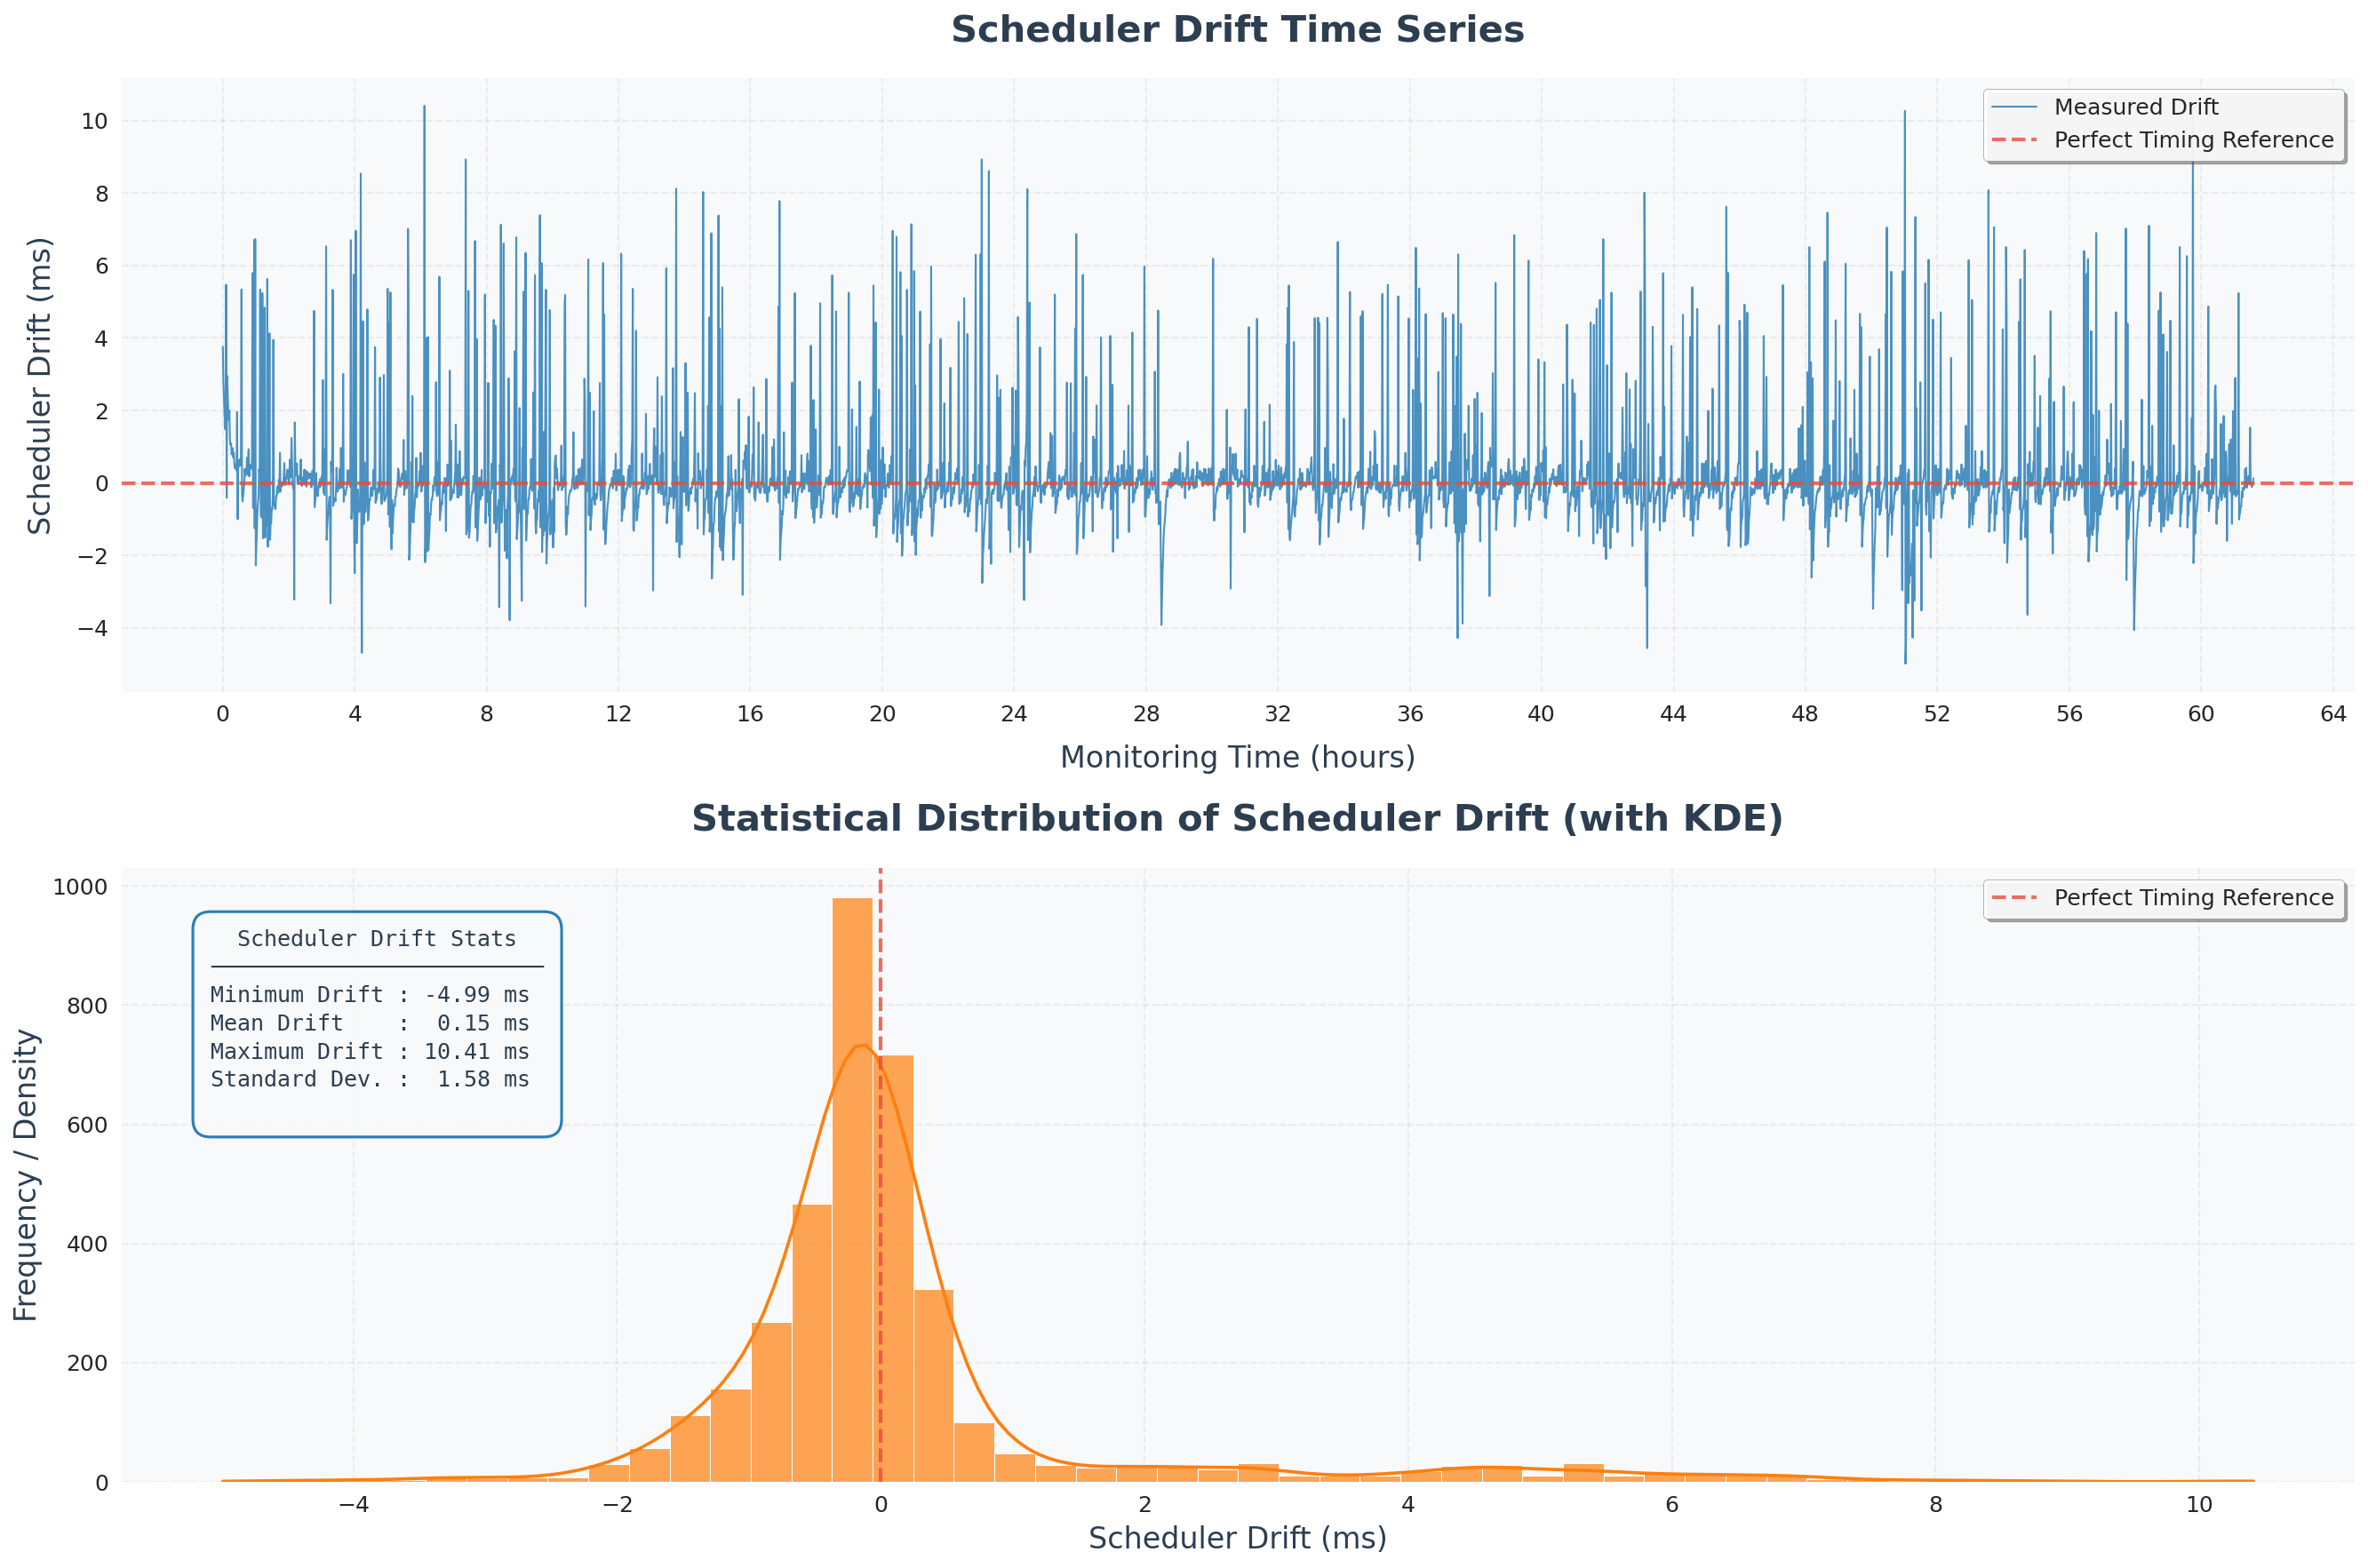
\includegraphics[width=\textwidth]{../plots/62-hours/scheduler_timing_drift_performance.png}
    \caption{Scheduler drift analysis: (a) temporal drift measurements over 62-hour period, (b) statistical distribution histogram with kernel density estimation overlay}
    \label{fig:scheduler_drift}
\end{figure}

The scheduler achieved exceptional timing precision with mean drift of 0.15 ms from intended minute boundaries. Statistical analysis reveals:

\begin{itemize}
    \item \textbf{Distribution Characteristics:} Near-Gaussian distribution with standard deviation of 1.58 ms indicates predictable behavior with minimal variance.

    \item \textbf{Symmetrical Distribution:} The drift distribution exhibits a nearly perfect Gaussian shape (normal distribution), demonstrating the effectiveness of the exponential moving average (EMA) compensation mechanism. This symmetry indicates that early and late completions are equally likely, with no systematic bias.
    
    \item \textbf{Asymmetric Tail Behavior:} While the distribution is largely symmetrical, there is a skew toward positive drift values in the extreme tail. This reflects the reactive nature of the EMA compensation: positive drift represents genuine load-induced delays, while negative drift results from overestimating execution time after load conditions improve, creating an bias toward positive extremes during load spikes.
    
    \item \textbf{Bounded Deviations:} Maximum positive drift of 10.41 ms and minimum of -4.99 ms remain well within acceptable soft real-time constraints of the application.
                    
    \item \textbf{Sub-millisecond Precision:} Over 50\% of cycles achieve sub-0.4 ms drift precision. This demonstrates exceptional performance of the EMA compensation.

    \item \textbf{Load Adaptation:} Transient drift spikes correlate with high message throughput periods, yet the EMA compensation mechanism ensures rapid recovery to baseline performance, demonstrating effective load balancing (see Section~\ref{sec:throughput_analysis}).

\end{itemize}

\subsection{Latency Analysis and Decomposition}

End-to-end latency analysis provides insights into system responsiveness and bottleneck identification. Figure~\ref{fig:latency_breakdown} decomposes total latency into network latency (exchange timestamp to local receipt) and processing latency (local receipt log completion) components.

\begin{figure}[H]
    \centering
    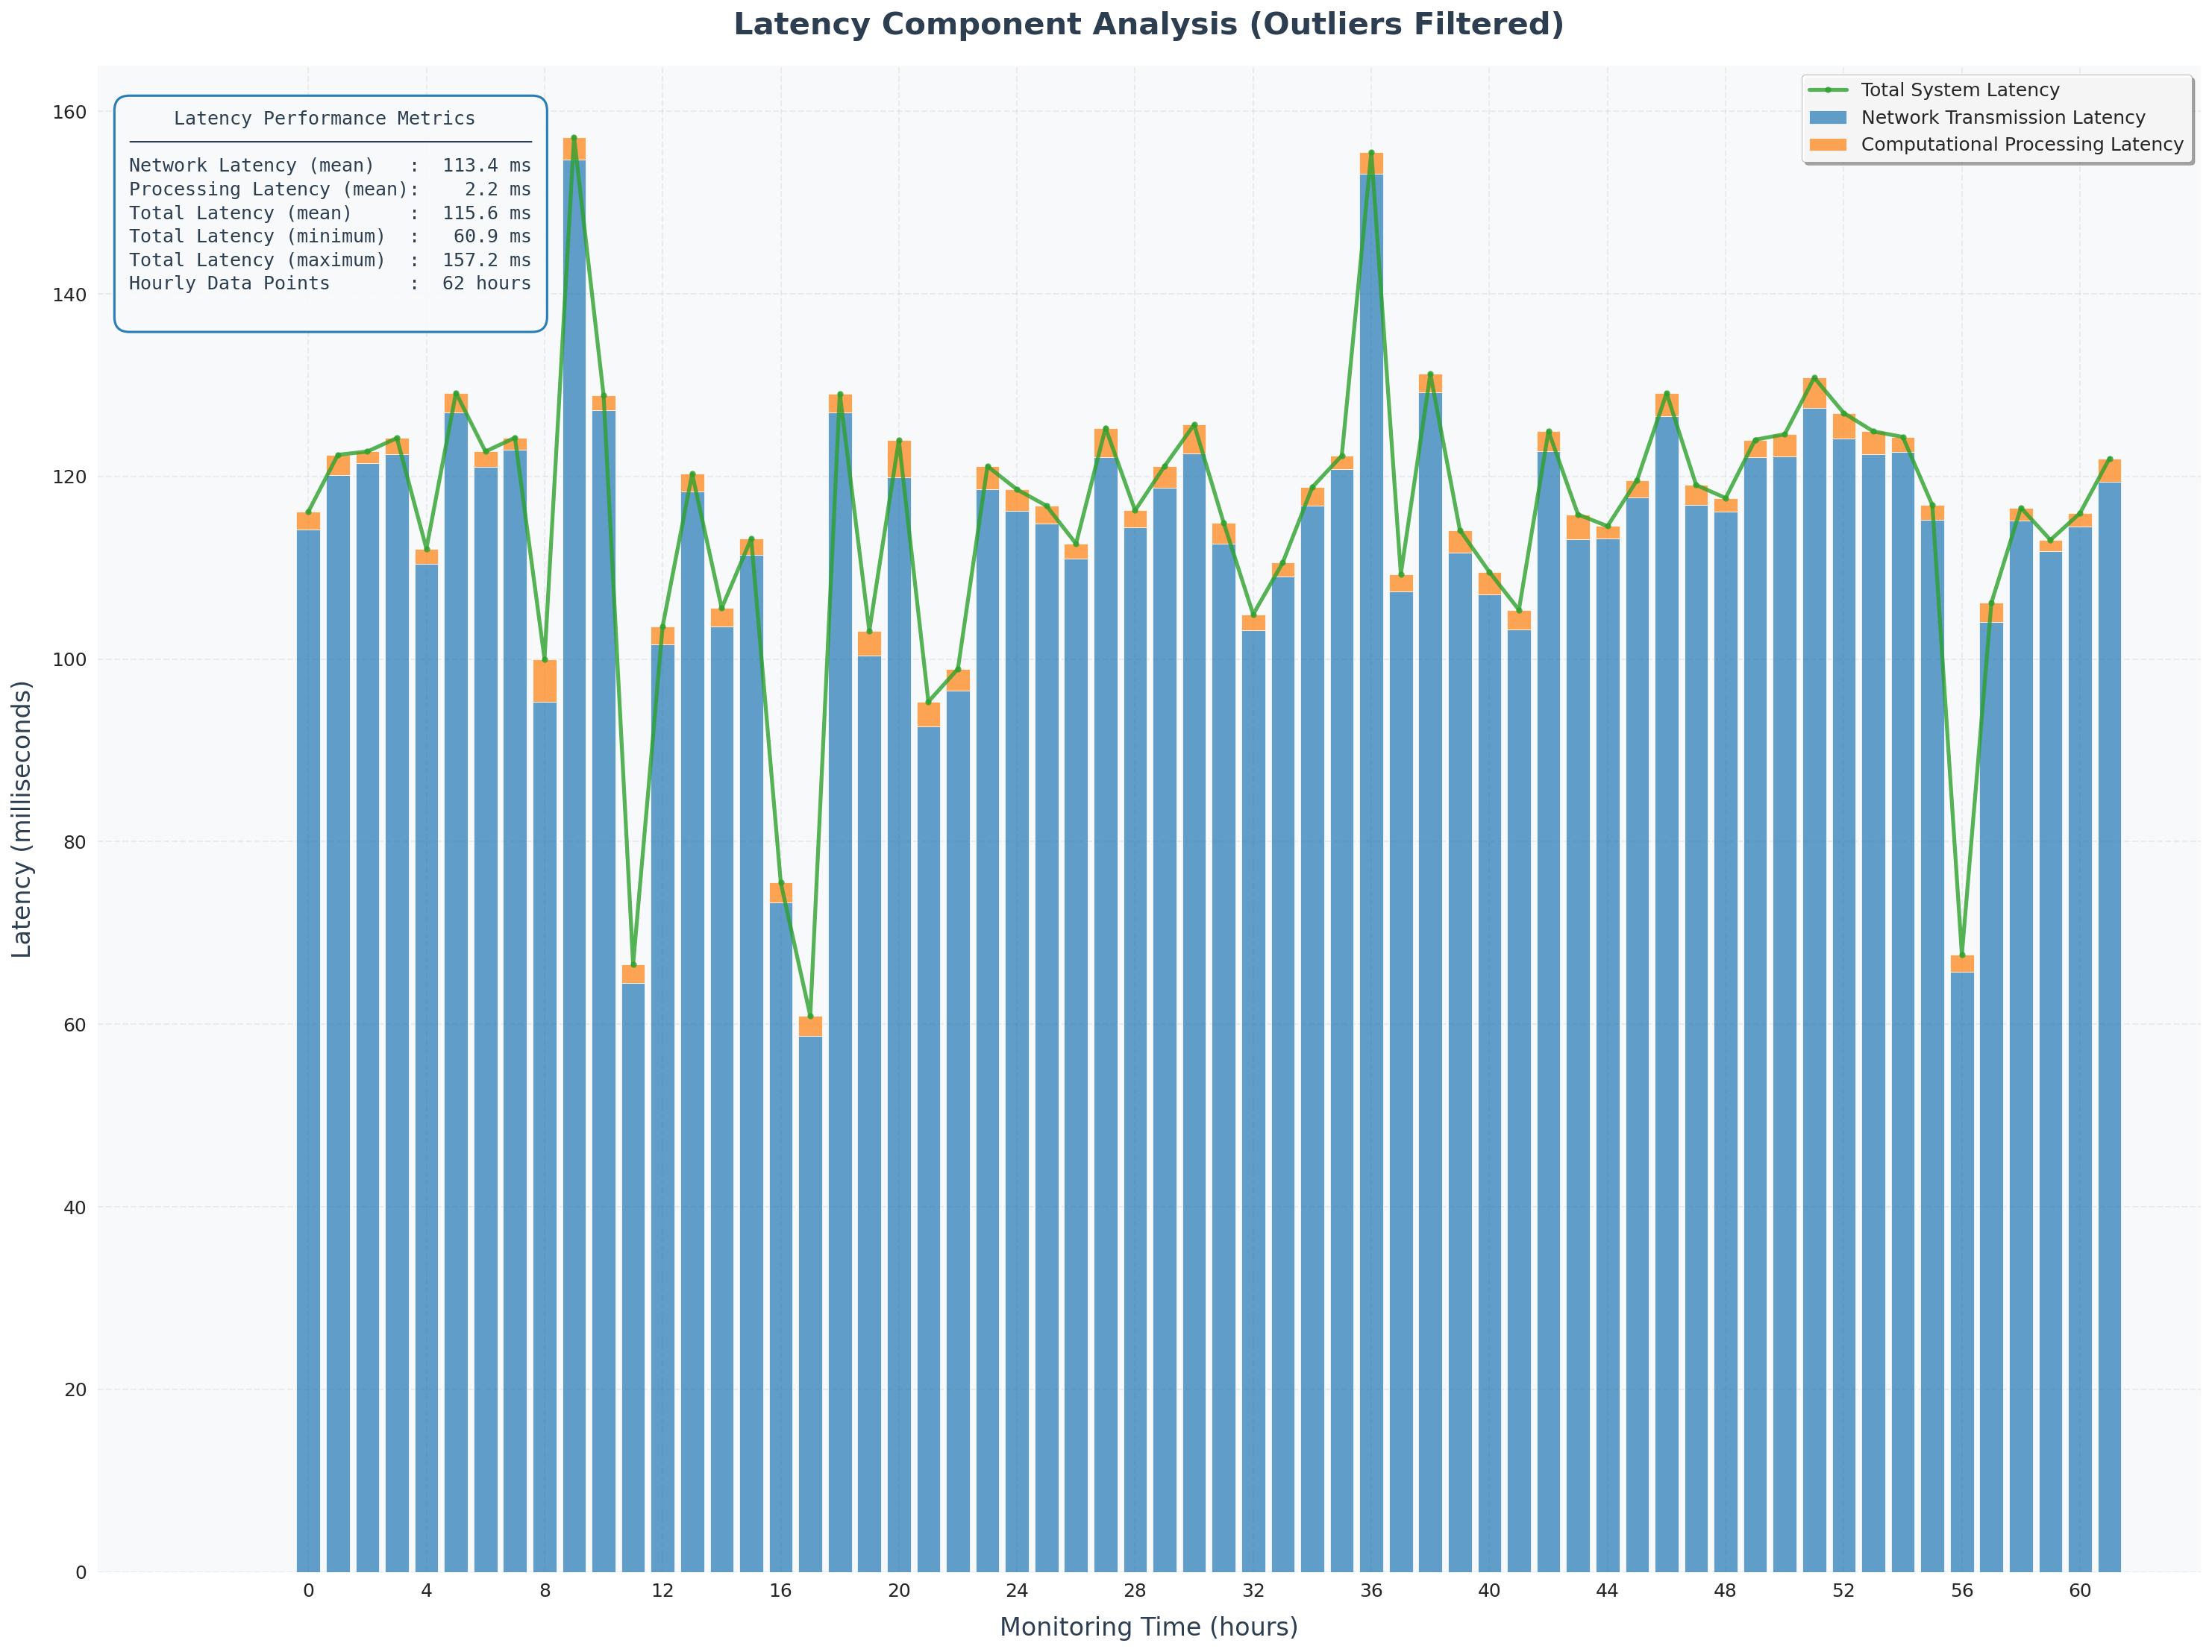
\includegraphics[width=\textwidth]{../plots/62-hours/network_processing_latency_breakdown.png}
    \caption{Latency Breakdown of network \& processing latency by hour (stacked bar chart)}
    \label{fig:latency_breakdown}
\end{figure}

Latency analysis reveals critical performance characteristics:

\begin{itemize}
    \item \textbf{Component Distribution:} Network latency dominates at 98\% of total latency, attributable to geographical distance between the Raspberry Pi and OKX servers.
    
    \item \textbf{Processing Efficiency:} Local processing maintains consistent 2.2 ms average latency, validating the effectiveness of the custom JSON parser and data structures.

    \item \textbf{Temporal Stability:} Both network and processing latencies remain stable throughout the monitoring period, with no systematic degradation over time.
    
    \item \textbf{Network Variability Patterns:} Network latency exhibits periodic variations ranging from 60-160 ms, attributable to internet traffic fluctuations, routing changes, and server load variations at the OKX exchange infrastructure. Analysis reveals a direct correlation between network conditions and market activity levels. At hour 8, both network latency and message throughput (the highest message rate of the entire monitoring period, see Figure~\ref{fig:cpu_vs_messages}) reach their simultaneous peaks. This indicates that periods of high trading activity systematically correlate with increased load on both OKX exchange infrastructure and intermediate network paths. Exchange servers experience elevated computational load during peak trading periods, contributing to increased response times, while concurrent high-frequency trading activity creates additional network congestion across internet backbone routes.

\end{itemize}

\subsection{Resource Utilization Analysis}

Embedded system constraints necessitate efficient resource management. Figure~\ref{fig:cpu_memory} illustrates CPU and memory utilization patterns.

\begin{figure}[H]
    \centering
    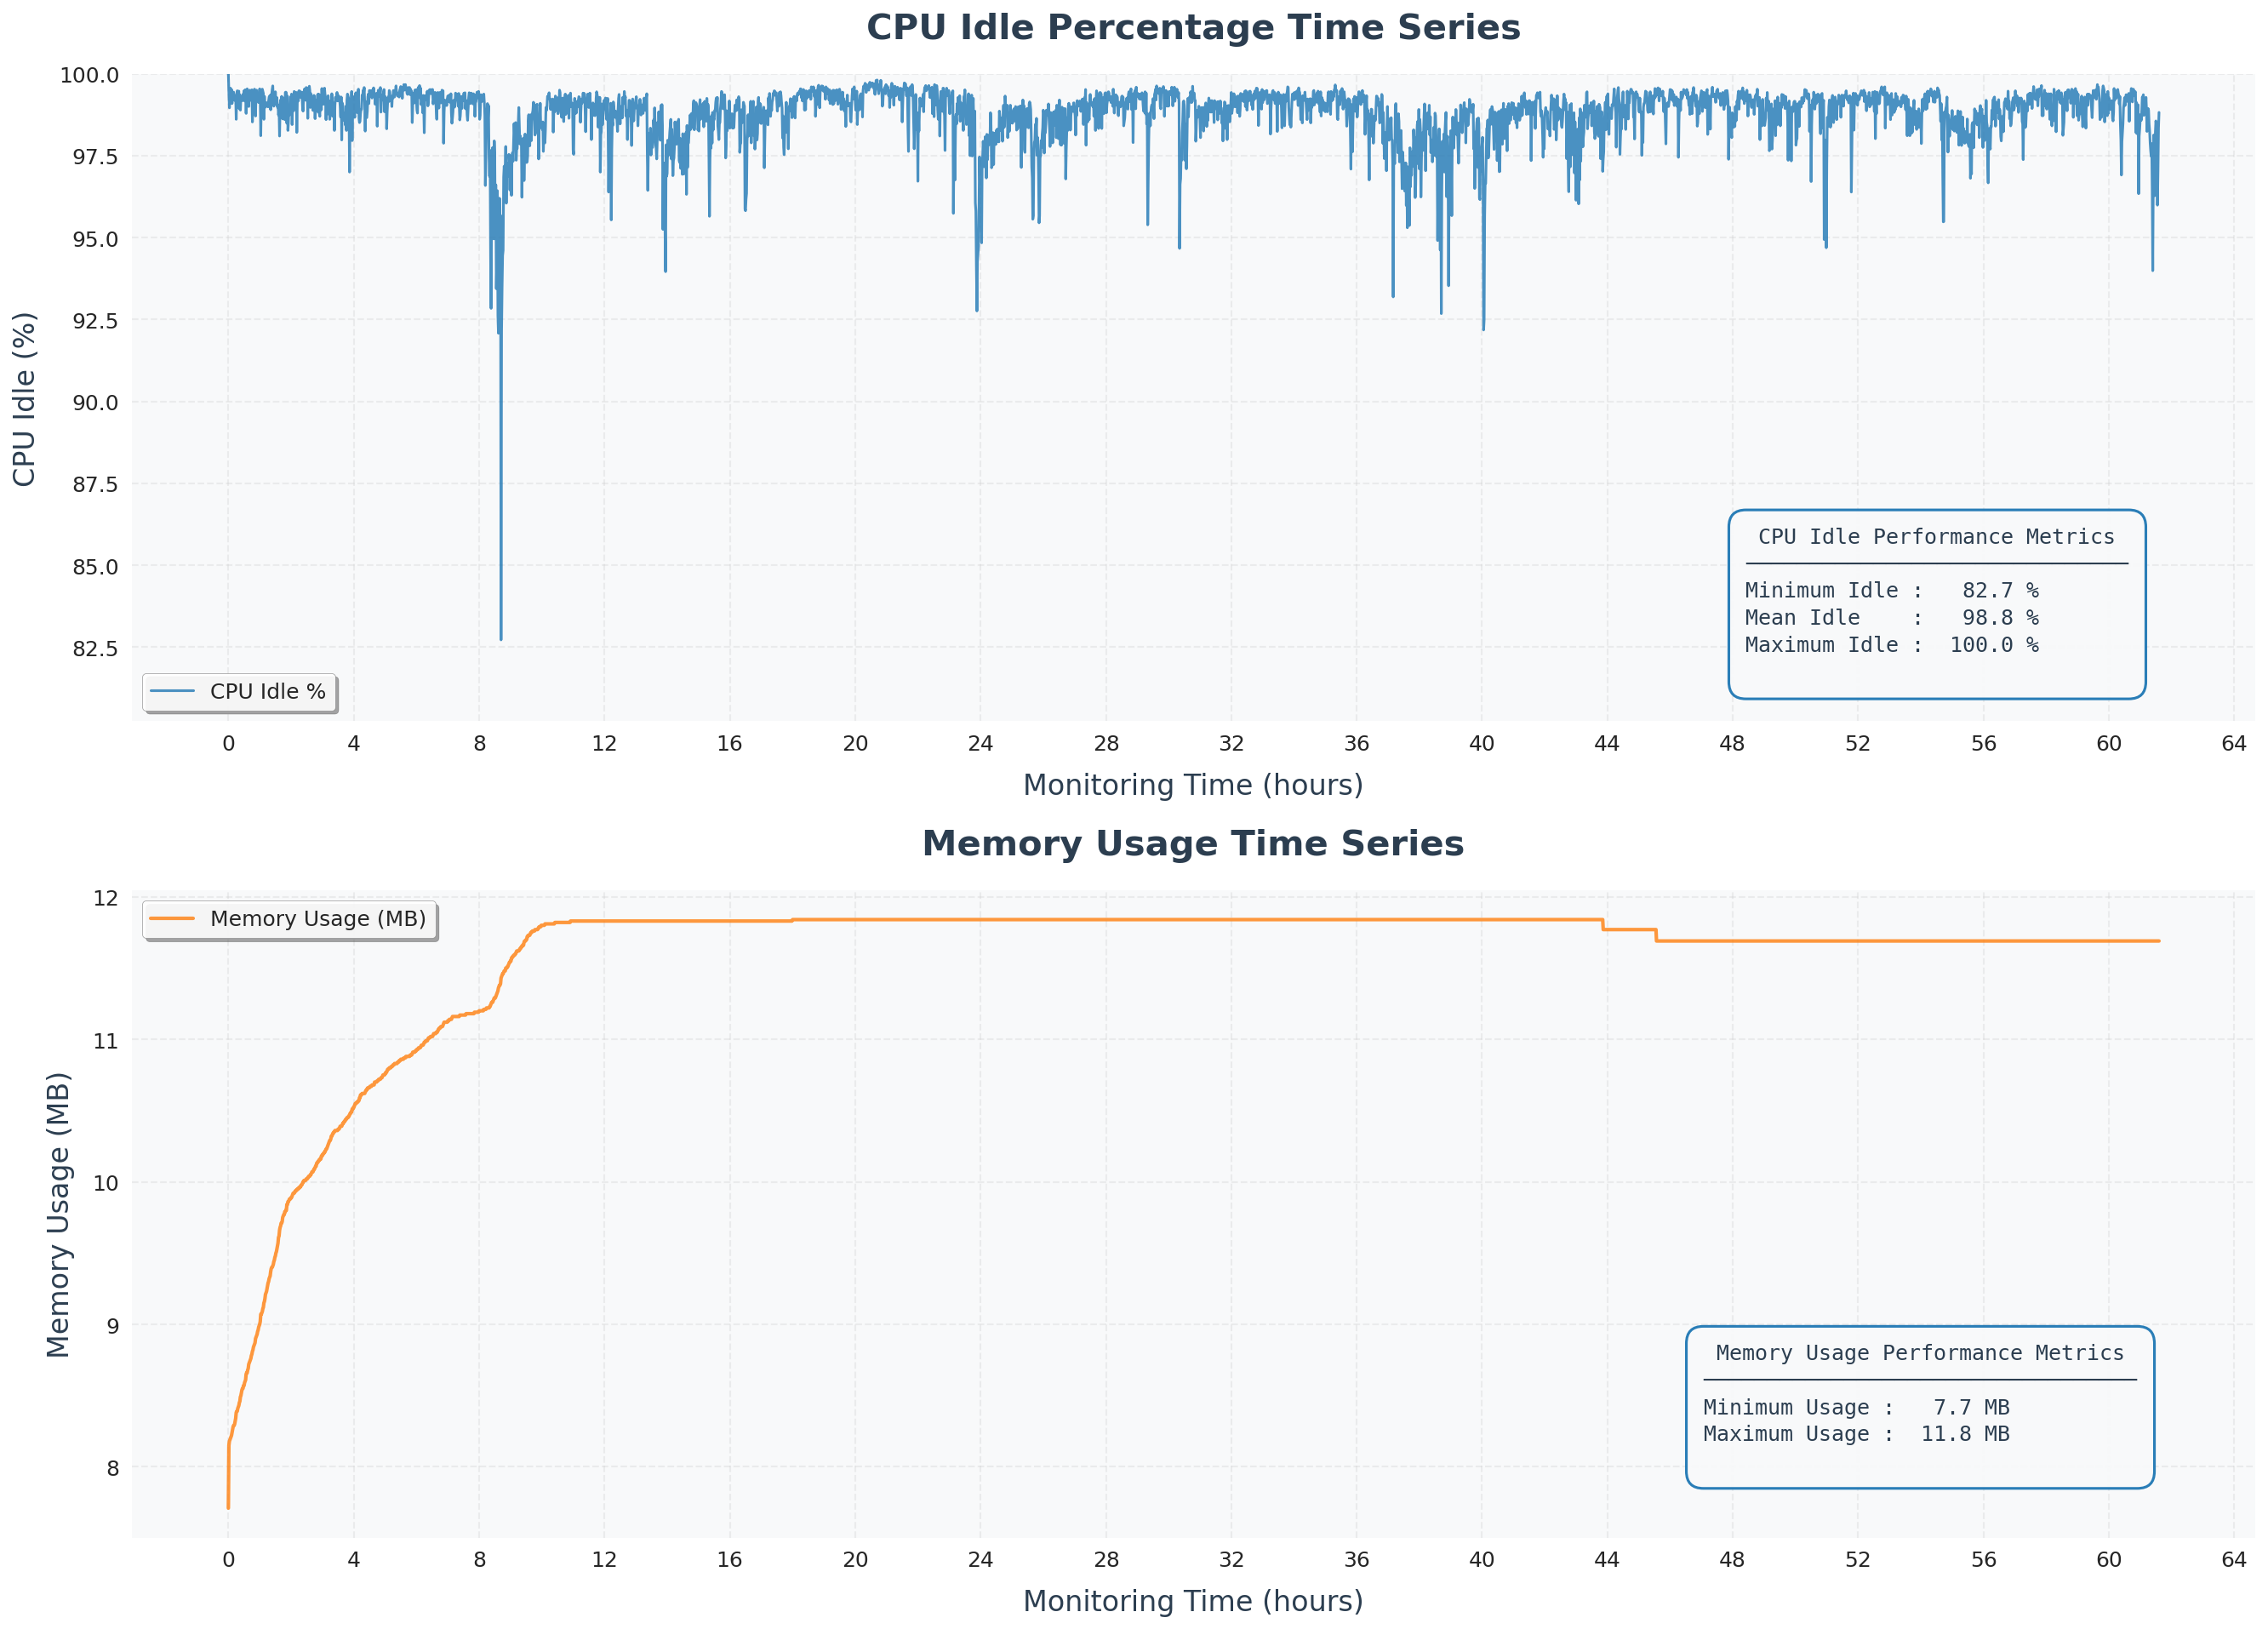
\includegraphics[width=\textwidth]{../plots/62-hours/system_resources_cpu_memory_usage.png}
    \caption{CPU Idle Time and Memory Usage over time}
    \label{fig:cpu_memory}
\end{figure}

Resource utilization demonstrates exceptional efficiency:

\begin{itemize}
    \item \textbf{CPU Efficiency:} Mean CPU idle time of 98.8\% indicates minimal processor load.
    
    \item \textbf{Memory Stability:} Memory usage rises sharply at startup due to pre-allocation of large buffers, then gradually increases as buffers are filled with live data. It plateaus at 11.8MB, confirming the absence of memory leaks.   
    \begin{itemize}
        \item \textbf{Progressive Physical Allocation (0-10 hours):} Virtual memory allocation via \texttt{calloc()} for all data structures, but only accessed pages appear in VmRSS. Gradual increase as circular buffers are written to for the first time, causing page faults that allocate physical memory        

        \item \textbf{Steady State (10+ hr):} Once all allocated pages have been touched, VmRSS stabilizes at the true memory footprint.

        \item \textbf{Memory Efficiency:} Only 2.3\% memory utilization (11.8 MB of 512 MB)
    \end{itemize}

\end{itemize}

\subsection{Throughput Scalability Analysis}
\label{sec:throughput_analysis}

System scalability was evaluated through correlation analysis between message processing rate and CPU utilization. Figure~\ref{fig:cpu_vs_messages} presents this relationship.

\begin{figure}[H]
    \centering
    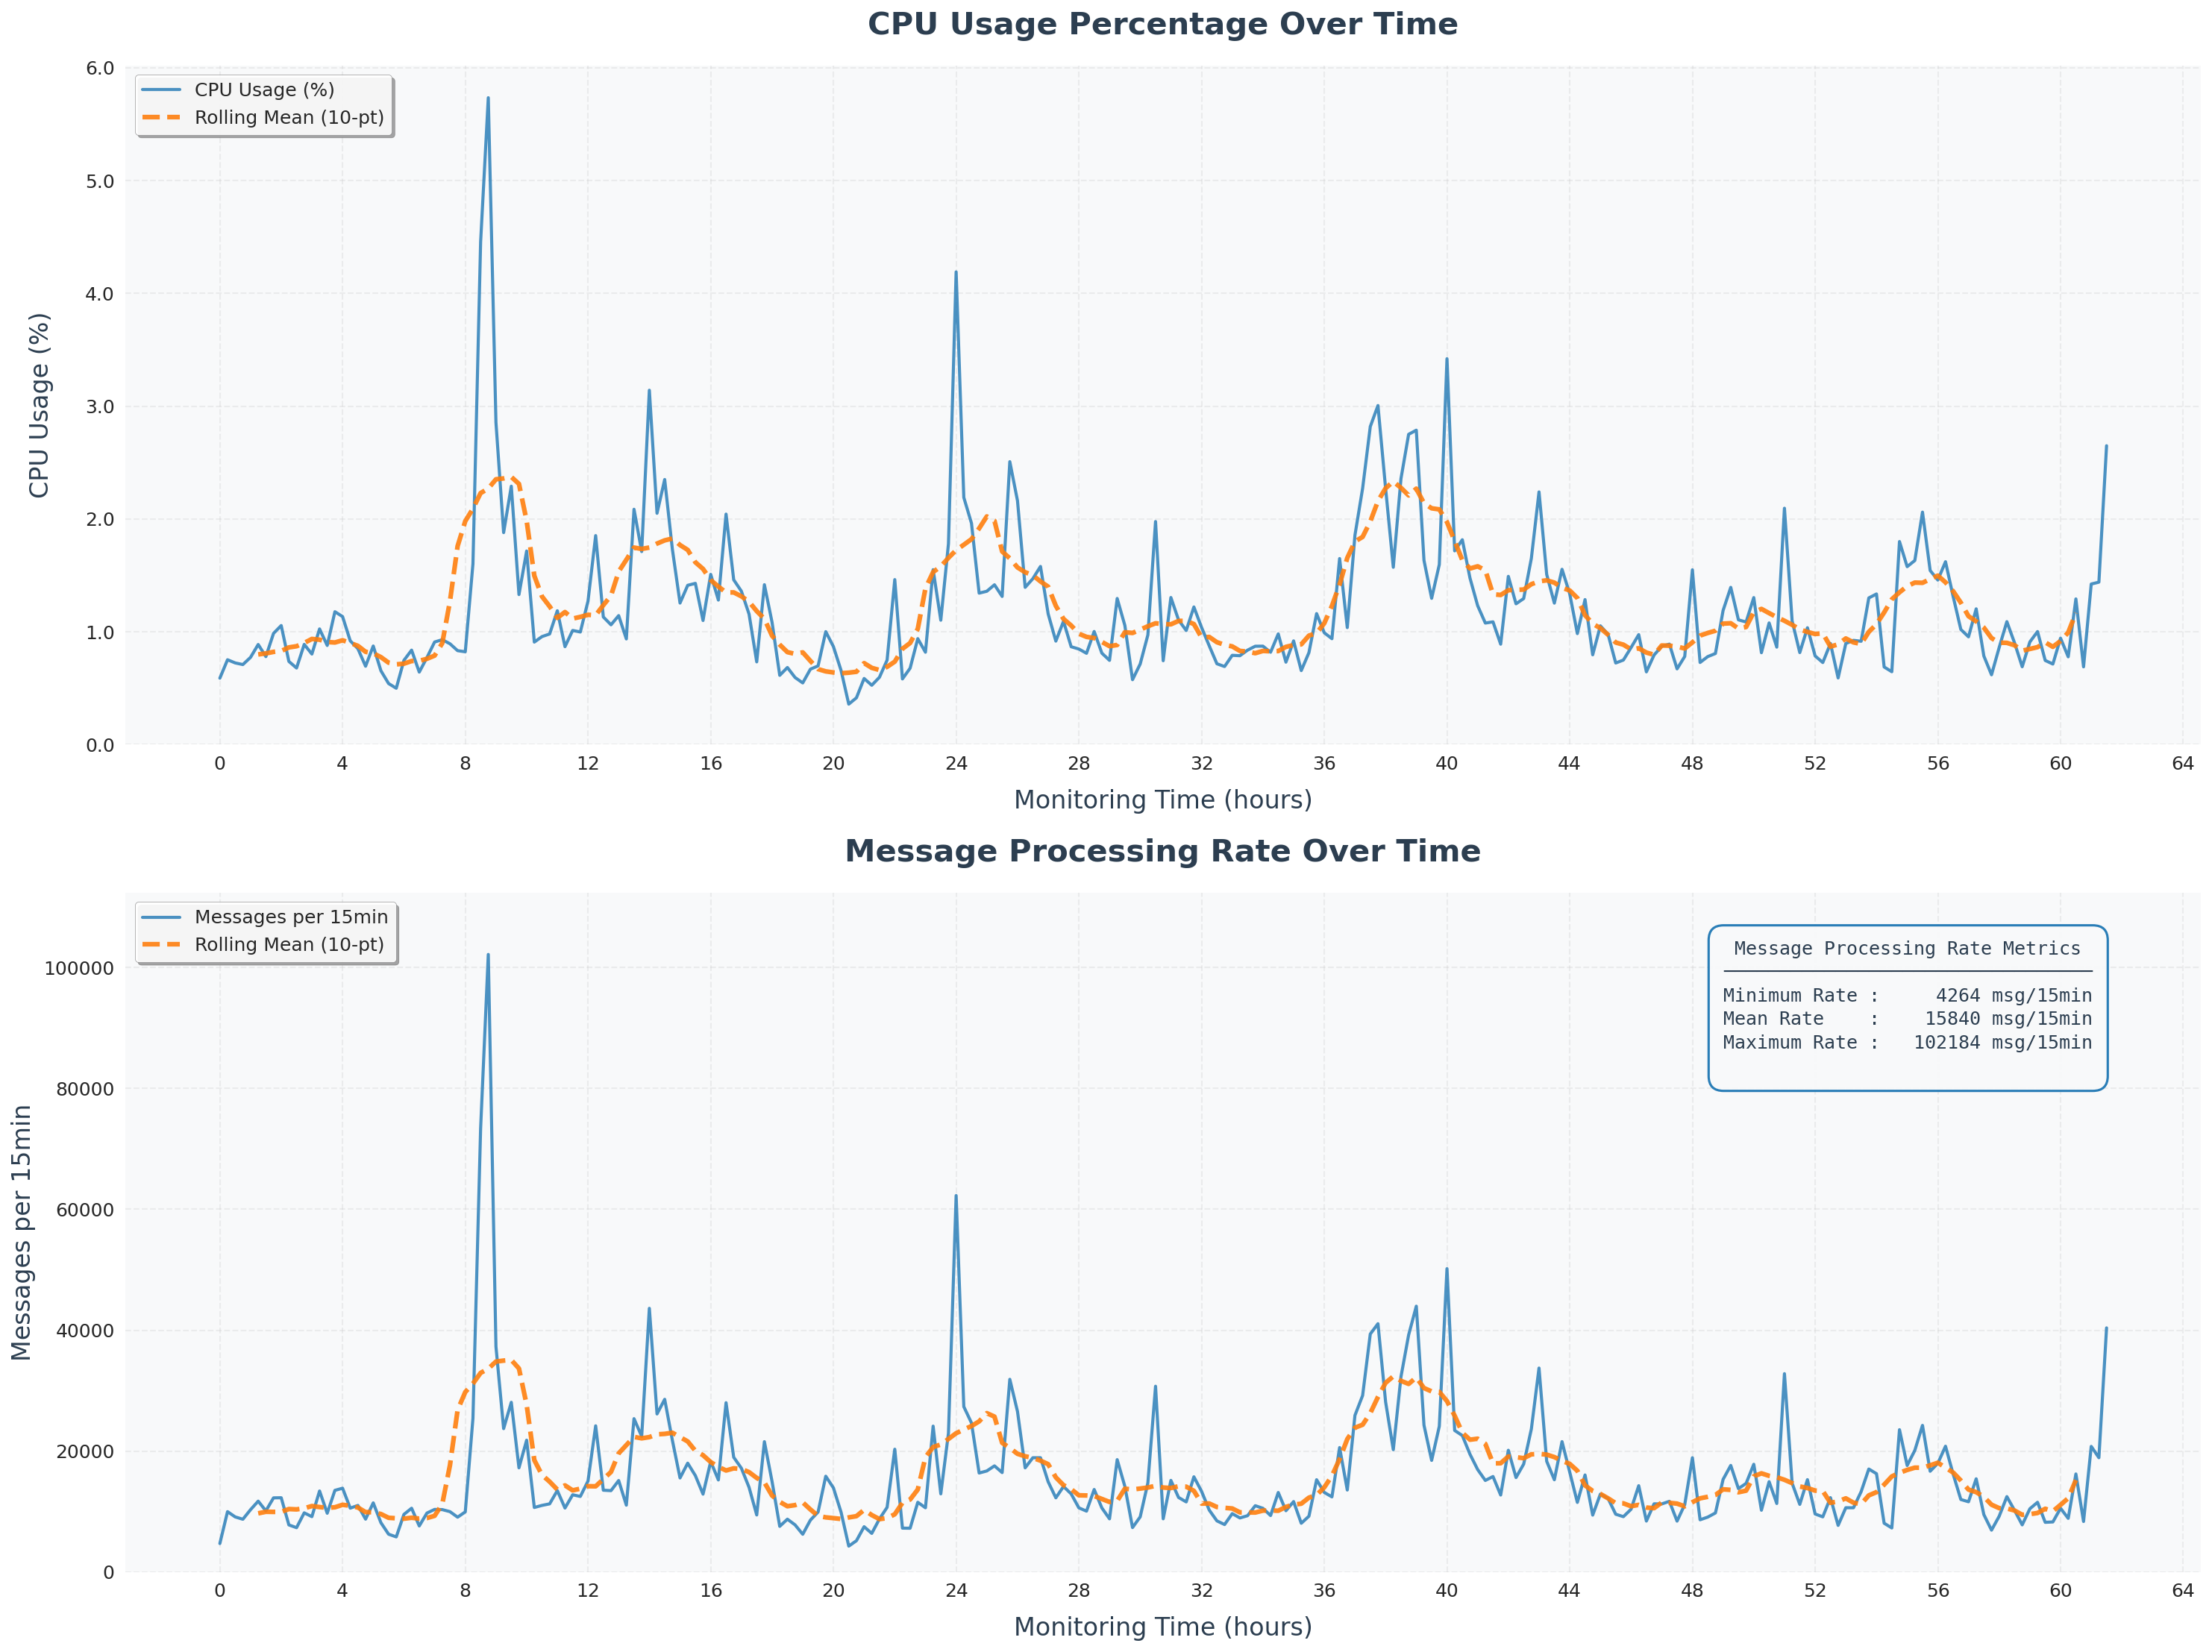
\includegraphics[width=\textwidth]{../plots/62-hours/cpu_load_vs_message_throughput.png}
    \caption{Correlation between message processing rate and CPU usage in 15-minute intervals. Top panel shows CPU usage percentage, bottom panel shows message throughput.}
    \label{fig:cpu_vs_messages}
\end{figure}

Scalability analysis yields significant insights:

\begin{itemize}
    \item \textbf{Strong Linear Correlation:} Pearson correlation coefficient of 0.98 between CPU usage and message rate confirms linear scaling characteristics.
    
    \item \textbf{Burst Handling:} The system successfully processes traffic bursts up to 102,184 messages per 15-minute window ($\approx 114$ msg/s) without performance degradation.        

    \item \textbf{Capacity Headroom:} With peak CPU usage at 7\% while processing 114 messages per second, theoretical capacity exceeds 1,600 messages per second before saturation.
    
\end{itemize}


\section{Technical Innovations and Optimizations}

\subsection{Minimal WebSocket Processing}
\label{sec:Minimal WebSocket Processing}

To minimize processing overhead and prevent data loss in the critical network path, the WebSocket callback is designed to perform only the absolute minimum work necessary. The WebSocket callback implements a \textbf{minimal processing approach} that eliminates parsing overhead and reduces critical section duration. Upon receiving each trade message, the callback executes the following optimized sequence:

\begin{itemize}
    \item \textbf{Immediate Timestamping:} Captures a high-resolution timestamp using \texttt{CLOCK\_REALTIME}, ensuring minimal delay between actual message receipt and temporal marking
    
    \item \textbf{Zero-Copy Buffer Management:} Rather than parsing the JSON payload within the callback context, the raw message is copied directly into a pre-allocated fixed buffer with a 1024-byte capacity limit
    
    \item \textbf{Thread-Safe Queuing:} The raw message, along with its receive timestamp, is pushed into a thread-safe ring buffer using mutex-protected queue operations
    
    \item \textbf{Deferred Processing:} All parsing, validation, and processing logic is deferred to a dedicated consumer thread operating outside the network callback context
\end{itemize}

This architectural approach delivers critical advantages:

\begin{itemize}
    \item \textbf{Minimal Blocking:} The WebSocket thread experiences minimal blocking, maintaining consistent network throughput even during computation-intensive periods
    
    \item \textbf{High Responsiveness:} By offloading all non-essential work to a separate thread, the system achieves exceptional responsiveness to incoming data streams        
\end{itemize}

\subsection{Optimized JSON Parsing with a Custom Parser}

Parsing the JSON payload is a frequent operation in the critical path. To minimize latency, we compared the standard \texttt{cJSON} library with a lightweight custom parser. The custom parser achieved an approximately \textbf{30\% performance improvement} in parsing speed. This gain comes from a zero-allocation design: instead of building an in-memory parse tree, the custom parser uses direct string operations (\texttt{strstr}, \texttt{strchr}) to locate required fields (\texttt{instId, px, sz, ts}) directly in the raw message buffer. 

However, this optimization involves a trade-off between performance and robustness:

\subsubsection*{Pros of the Custom Parser}
\begin{itemize}
    \item \textbf{High Performance:} By avoiding the overhead of a general-purpose parsing state machine and dynamic memory allocations, the custom parser is significantly faster.
    \item \textbf{Minimal Memory Footprint:} Operates on the existing buffer with only stack-allocated output, reducing heap usage and fragmentation.
    \item \textbf{No External Dependencies:} It removes the need to link against the \texttt{cJSON} library, resulting in a smaller binary and a simpler build process.
\end{itemize}

\subsubsection*{Cons of the Custom Parser}
\begin{itemize}
    \item \textbf{Fragility:} The parser is brittle and tightly coupled to the exact OKX trade message format. Any changes in field ordering or formatting could break it.
    \item \textbf{Limited Error Handling:} It is not a fully compliant JSON parser and may fail on malformed input. A full library like \texttt{cJSON} provides more robust error checking.
\end{itemize}

For this specific application, where the input format is well-defined and performance on a resource-constrained device is paramount, the trade-off is justified. The 30\% speed gain directly contributes to lower processing latency and higher system throughput.

\subsection{Concurrency for I/O Optimization on a Single Core}
\label{sec:Concurrency on Single Core}

A key architectural decision was to separate the per-minute computations (VWAP and Correlation) into two distinct worker threads coordinated by a scheduler, rather than executing them sequentially in a single thread. On a multi-core processor, the benefits of such parallelism are obvious. However, on the single-core Raspberry Pi Zero W, this design still yielded a significant \textbf{15\% decrease in scheduler drift time}. This counter-intuitive result is not due to parallelism, but to the efficient use of concurrency to hide I/O latency.

The primary reason for this performance gain is the \textbf{overlapping of I/O-bound and CPU-bound work}. Both tasks follow a \texttt{compute-then-write} pattern:
\begin{itemize}
    \item \textbf{Compute (CPU-bound):} Calculate VWAP or Pearson correlation.
    \item \textbf{Write (I/O-bound):} Save results to an SD card file.
\end{itemize}

File writes block the thread while the disk completes the operation. In a sequential model, the thread would compute VWAP, block on its file write, then compute correlation, then block again. The CPU remains idle during each write. In our multi-threaded model, when the VWAP worker blocks on a write, the scheduler switches to the correlation worker, which can compute its results during the first thread’s I/O wait. This overlapping of one thread’s I/O wait with another’s CPU work leads to more effective CPU utilization and a shorter total wall-clock time. It demonstrates that concurrency can mask I/O latency, an important optimization for real-time systems on embedded hardware.

\subsection{Memory Optimization}

Operating within the 512MB RAM constraint of the Raspberry Pi Zero W requires careful memory management to prevent fragmentation and corruption during extended execution periods. The system employs several memory optimization strategies:

\begin{itemize}

\item \textbf{Pre-allocated circular buffers with fixed capacity:} All data structures utilize static memory allocation determined at system initialization, completely eliminating runtime \texttt{malloc()}/\texttt{free()} operations. This design avoids the heap fragmentation risks associated with dynamic data structures (such as linked lists requiring per-node allocation) that could cause memory exhaustion during extended operation periods.

\item \textbf{Elimination of memory leaks:} Static allocation eliminates the risk of memory leaks. In garbage-collected languages, automatic memory management handles this, but C requires manual memory management that becomes error-prone.

\item \textbf{Deterministic memory usage:} Pre-allocated buffers provide predictable, constant memory footprint essential for embedded systems, preventing unpredictable memory growth that could exceed system constraints during peak loads.
\end{itemize}

\subsection{File I/O Performance Optimization}

Frequent file writes can introduce latency and block processing, creating bottlenecks in the real-time data pipeline. The system addresses this through a configurable \texttt{fsync()} policy that provides a trade-off mechanism between data durability and real-time performance.

File descriptors are kept open throughout the entire system lifecycle to minimize the overhead of repeated open/close operations. This approach eliminates the syscall overhead that would otherwise occur with each write operation, while the configurable \texttt{fsync()} setting allows deployment-specific optimization based on reliability requirements.

\textbf{Performance Impact Analysis}

\begin{itemize}
\item \textbf{With fsync enabled:} Processing time averaged 100ms per operation
\item \textbf{With fsync disabled:} Processing time reduced to approximately 2ms per operation
\item \textbf{Performance improvement:} 98\% reduction in processing latency
\end{itemize}

This substantial improvement occurs because \texttt{fsync()} forces immediate synchronization of buffered data to the underlying SD card storage, which is inherently slow due to the mechanical nature of flash memory operations. Without \texttt{fsync()}, writes are buffered by the kernel's page cache and flushed asynchronously through the operating system's write-back mechanism, allowing the application to continue processing immediately without blocking on storage hardware.

For applications requiring maximum data durability, \texttt{fsync()} can be enabled by setting FSYNC\_PER\_WRITE to 1, on line 67 in \texttt{include/common.h}. However, this configuration significantly impacts real-time performance and should be carefully considered based on the specific reliability requirements of the deployment environment.

\paragraph{Trade-offs and Risk Assessment:} While disabling \texttt{fsync()} provides exceptional performance gains, it introduces potential data durability risks that must be carefully evaluated. In the event of unexpected system shutdown or power loss, recently written data residing in kernel buffers may be lost before being committed to persistent storage.

\section{Conclusion}

We have demonstrated a real-time transaction processing system in C on a Raspberry Pi Zero W that ingests cryptocurrency trade data and computes live analytics under strict timing constraints. The system achieved all specified requirements while maintaining exceptional performance characteristics:

\begin{enumerate}
    \item \textbf{Real-Time Performance:} Sub-ms processing latency with 96.8\% CPU idle time
    \item \textbf{Timing Precision:} Drift-free minute-boundary scheduling with 0.15ms ms accuracy
    \item \textbf{Memory Efficiency:} Stable 11 MB memory usage within the 512 MB constraint
\end{enumerate}    

The implementation validates that sophisticated financial data processing applications can be effectively deployed on embedded platforms through careful architectural design, optimized data structures, and precise scheduling mechanisms.


\section{Future Work}

Potential enhancements to extend system capabilities include:
\begin{itemize}
    \item \textbf{Advanced Statistical Models:} Implementation of Spearman rank correlation and mutual information metrics for non-linear relationship detection
    \item \textbf{Machine Learning Integration:} Deployment of lightweight neural networks for real-time price prediction and anomaly detection
    \item \textbf{Data Compression:} Apply compression for long-term storage of logs and metrics.
\end{itemize}

\begin{thebibliography}{3}
    \bibitem{okx-api}
    OKX, \href{https://www.okx.com/docs-v5/en/#websocket-api-public-channel}{WebSocket API Documentation}.
    
    \bibitem{libwebsockets}
    Libwebsockets, \href{https://libwebsockets.org/}{C Library for WebSocket Clients and Servers}.
    
    \bibitem{project-repo}
    GitHub Repository, \href{https://github.com/fraidakis/realtime-embedded-crypto-processor}{Real-Time Transaction Processing System Source Code}.
\end{thebibliography}

\newpage

\pagenumbering{roman}

\begin{appendices}
\section{Data Format Specifications}

\subsection{Trade Log Format}
Raw OKX WebSocket messages in JSON Lines format:
\begin{verbatim}
{"arg":{"channel":"trades","instType":"SPOT","instId":"BTC-USDT"},
 "data":[{"instId":"BTC-USDT","tradeId":"123456789",
          "px":"27345.67","sz":"0.12345","ts":"1694464949239"}]}
\end{verbatim}

\subsection{VWAP Output Format}
CSV format with ISO 8601 timestamps:
\begin{verbatim}
timestamp_iso,vwap,volume
2025-10-01T01:08:00+0100,4148.77269479,25.579497
\end{verbatim}

\subsection{Correlation Output Format}
CSV format with correlation coefficients and lag timestamps:
\begin{verbatim}
timestamp_iso,correlated_with,correlation,lag_timestamp_iso
2025-10-01T01:16:00+0100,ETH-USDT,0.960313,2025-10-01T01:15:00+0100
\end{verbatim}

\subsection{Performance Metrics Format}
System performance data in CSV format:
\begin{verbatim}
# system.csv
timestamp_ms,cpu_percent,memory_mb
1759277340000,0.58,11.69

# scheduler.csv
scheduled_ms,actual_ms,drift_ms
52380000,52380003,0.15

# latency.csv
symbol_idx,exchange_ts,recv_ts,process_ts,network_lat,process_lat,total_lat
1,1759277298329,1759277298437,1759277298438,108,1,109
\end{verbatim}


\end{appendices}

\end{document}